% This example is meant to be compiled with lualatex or xelatex
% The theme itself also supports pdflatex
\PassOptionsToPackage{unicode}{hyperref}
\documentclass[aspectratio=1610, 9pt]{beamer}

% Load packages you need here
\usepackage{polyglossia}
\setmainlanguage{german}

\usepackage{csquotes}
\usepackage{siunitx}
\usepackage{subfigure}

\usepackage{amsmath}
\usepackage{amssymb}
\usepackage{mathtools}

\usepackage{hyperref}
\usepackage{bookmark}

% load the theme after all packages

\usetheme[
  showtotalframes, % show total number of frames in the footline
]{tudo}

% Put settings here, like
\unimathsetup{
  math-style=ISO,
  bold-style=ISO,
  nabla=upright,
  partial=upright,
  mathrm=sym,
}

\title{Entwicklung eines Programmes zur Berechnung von Annealingeffekten in bestrahltem Silizium nach dem Hamburger Modell}
\author[C.~Krause]{Christopher Krause}
\institute[E4]{Experimentelle Physik \\ Fakultät Physik}
\titlegraphic{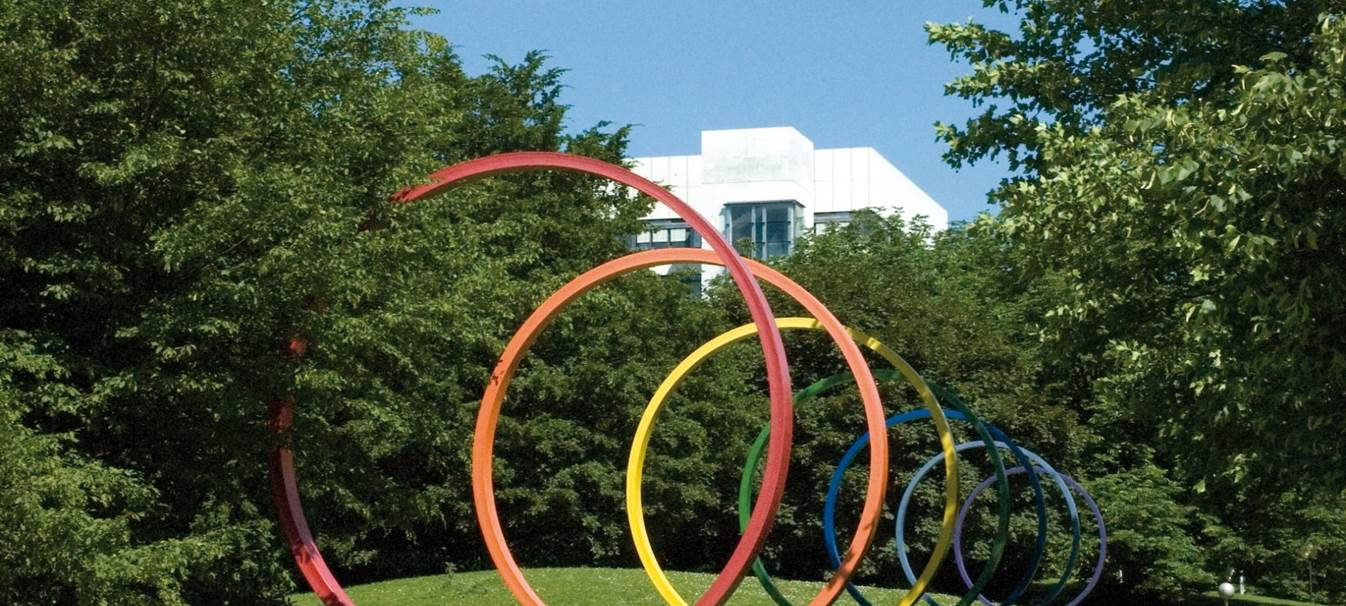
\includegraphics[width=0.7\textwidth]{images/tudo-title-2.jpg}}


\begin{document}

\maketitle

\begin{frame}{Ziel der Bachelorarbeit}
  Für beliebige Zeiten, Temperaturverläufe, Fluenzen und Materialeigenschaften:
  \begin{itemize}
    \item Berechnung der Dotierungskonzentration $\Delta N_{\mathrm{eff}}$
    \item Berechnung der Schadensrate $\alpha$
  \end{itemize}
  \medskip

  Zusätzliche Aufgaben:
  \begin{itemize}
    \item Interpolation der Daten für mehr und genauere Werte
    \item Erstellung eines Interfaces zur schnellen Berechnung von $\Delta N_{\mathrm{eff}}$ und $\alpha$
    für konstante Temperaturen
    \item Zusammenfügen von Datendateien und Anpassung der zugehörigen Zeiten
    \item Gesamte Annealinghistorie einer Diode berechnen
  \end{itemize}

\end{frame}

\begin{frame}{Theoretische Grundlage: Das Hamburg Modell}
  Die Änderung der Dotierungskonzentration bei annealing wird durch 3 Terme beschrieben:
  \medskip
  \begin{itemize}
    \item Stable damage:\: $N_{\mathrm{C}}(\Phi_{\mathrm{eq}}) = N_{\mathrm{C0}}[1-\exp{(-c \cdot \Phi_{\mathrm{eq}})}] + g_{\mathrm{c}} \cdot \Phi_{\mathrm{eq}}$
    \medskip
    \item Shortterm annealing:\: $N_{\mathrm{A}}(t, \Phi_{\mathrm{eq}}, T)= \Phi_{\mathrm{eq}} \cdot g_{\mathrm{a}} \cdot \exp{(-\frac{t}{\tau_{\mathrm{a}}})}$
    \medskip
    \item Longterm annealing:\: $N_{\mathrm{Y}}(t, \Phi_{\mathrm{eq}}, T)= \Phi_{\mathrm{eq}} \cdot g_{\mathrm{Y}} \cdot \left(1-\frac{1}{1+\frac{t}{\tau_{\mathrm{Y}}}}\right)$
    \medskip
    \item   $\Delta N_{\mathrm{eff}} = N_{\mathrm{C}}(\Phi_{\mathrm{eq}}) + N_{\mathrm{A}}(t, \Phi_{\mathrm{eq}}, T) + N_{\mathrm{Y}}(t, \Phi_{\mathrm{eq}}, T)$
  \end{itemize}
\end{frame}

\begin{frame}{Theoretische Grundlage: Das Hamburg Modell}
  Die Schadensrate wird bei annealing durch 2 Terme beschrieben:
  \medskip
  \begin{itemize}
    \item Shortterm annealing:\: $\alpha_I \cdot \exp{\left(-\frac{t}{\tau_{\mathrm{I}}(T)}\right)}$
    \medskip
    \item Longterm annealing:\: $\alpha_{\mathrm{0}}^{*} -\beta \cdot \ln{\left(\Theta(T) \cdot \frac{t}{t_{\mathrm{0}}}\right)}$, \:\:\: mit \: $\Theta(T) = \frac{E_{\mathrm{I}}^*}{k_b} \exp{\left(-\frac{1}{T}-\frac{1}{T_{\mathrm{ref}}}\right)}$
    \medskip
    \item $\alpha(t, T) = \alpha_I \cdot \exp{\left(-\frac{t}{\tau_{\mathrm{I}}(T)}\right)} + \alpha_{\mathrm{0}}^{*} -\beta \cdot \ln{\left(\Theta(T) \cdot \frac{t}{t_{\mathrm{0}}}\right)}$
  \end{itemize}
  \medskip

\end{frame}

\begin{frame}{Dotierungskonzentration für konstante Temperatur}
  \begin{figure}
      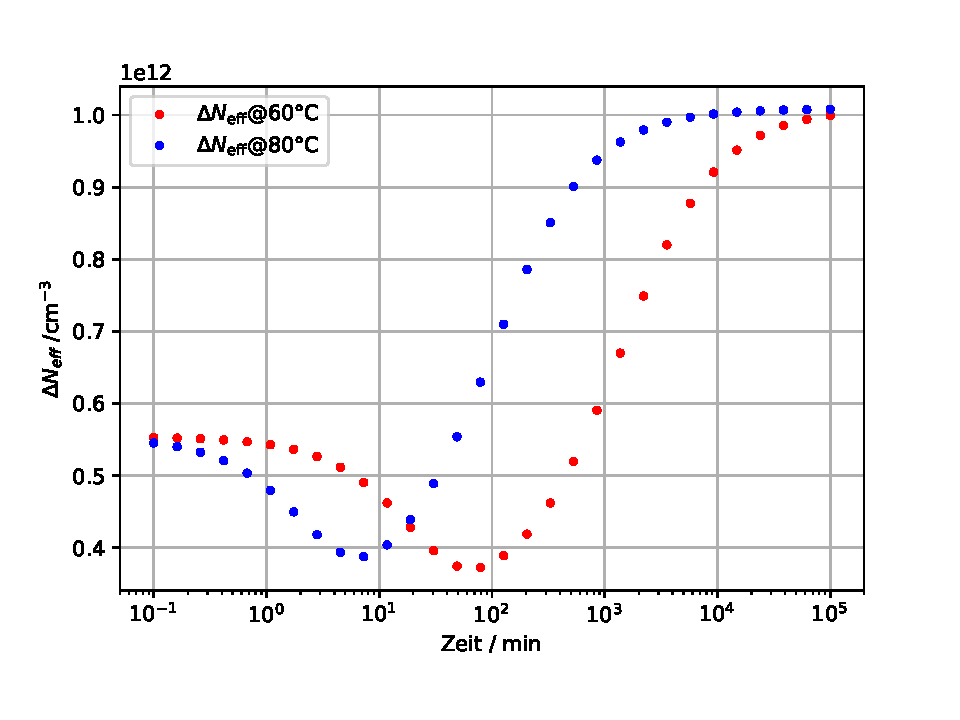
\includegraphics[width=0.55\textwidth]{images/annealing.PDF}
  \caption{$\Delta N_{eff}$ einer WE-25k Diode nach Bestrahlung mit Fluenz $\Phi_{\mathrm{eq}} = \SI{5e15}{\per\centi\meter\squared}$}
  \end{figure}
\end{frame}

\begin{frame}{Schadensrate für konstante Temperatur}
  \begin{figure}
      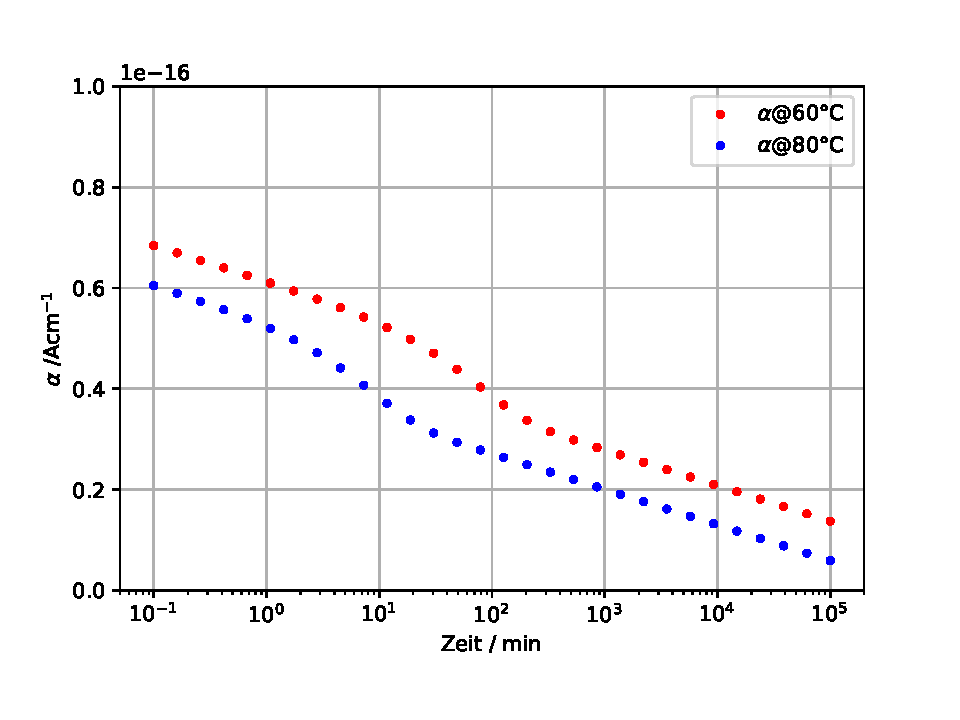
\includegraphics[width=0.55\textwidth]{images/damage.PDF}
  \caption{Schadensrate einer WE-25k Diode}
  \end{figure}
\end{frame}


\begin{frame}{Dotierungskonzentration für eine Temperaturkurve}
  \begin{figure}
      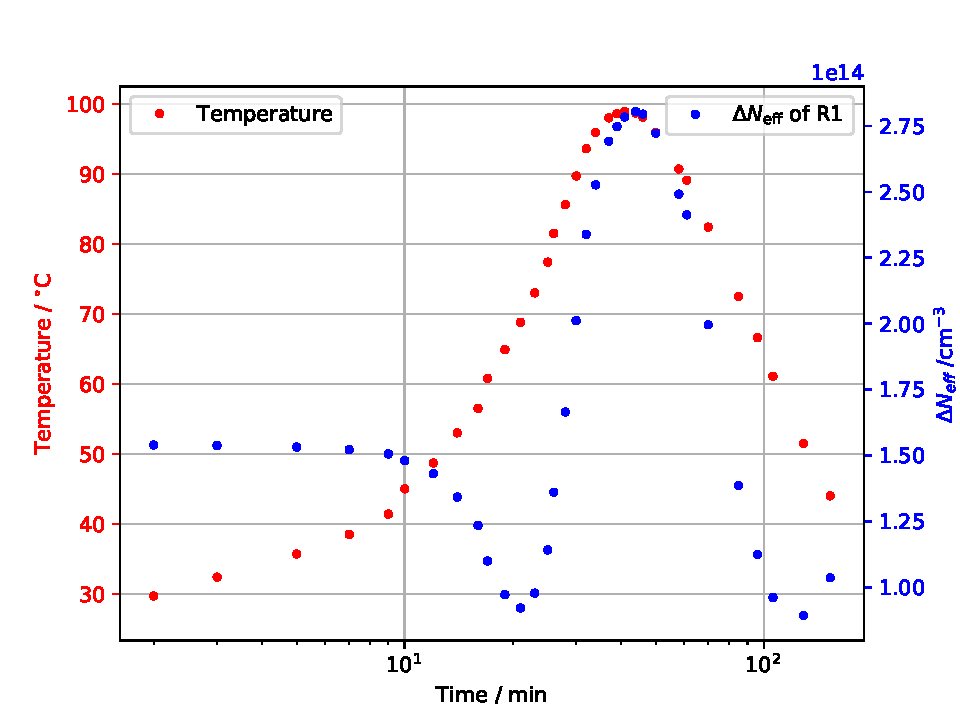
\includegraphics[width=0.55\textwidth]{images/ohnekorrektur.PDF}
  \caption{Dotierungskonzentration bei gleicher Fluenz und nicht konstanter Temperatur}
  \end{figure}
\end{frame}

\begin{frame}{Korrekturansatz}
  \begin{itemize}
    \item longterm annealing weist klare Abweichung vom eigentlichen Verhalten auf
    \medskip
    \item vorherige Temperaturänderungen werden vernachlässigt
    \medskip
    \item Funktion kann nur mit konstanter Temperatur rechnen
  \end{itemize}
  \medskip
  $\rightarrow$ Korrektur wird benötigt
  \medskip

  Ansatz: Über den Zeitraum $t_{\mathrm{i}} - t_{\mathrm{i-1}}$ wird mit der Temperatur $\frac{T_{\mathrm{i}} +T_{\mathrm{i-1}}}{2}$ erhitzt.

  Für den shortterm annealingeffekt gilt beispielsweise:
  \begin{align*}
    &\frac{t_{\mathrm{n}}}{\tau_{\mathrm{a}}(T_{\mathrm{n}})} \rightarrow \sum_{i=0}^n  \frac{t_{\mathrm{i}} - t_{\mathrm{i-1}}}{\tau_{\mathrm{a}}(\frac{T_{\mathrm{i}} +T_{\mathrm{i-1}}}{2})} \:\:\:\: \text{für} \: n>0 \\
    \\
    &\text{mit} \:\:\:\:\:\: \tau_{\mathrm{a}}(T) \propto \frac{1}{\exp{\left(-\frac{1}{T}\right)}} \\
    \\
    &\text{und}  \:\:\:\:\:\: N_{\mathrm{A}}(t, \Phi_{\mathrm{eq}}, T)     \propto \Phi_{\mathrm{eq}} \cdot \exp{\left(-\frac{t}{\tau_{\mathrm{a}}(T)}\right) }
  \end{align*}
\end{frame}

\begin{frame}{Dotierungskonzentration mit Korrektur}
  \begin{figure}
      \subfigure[]{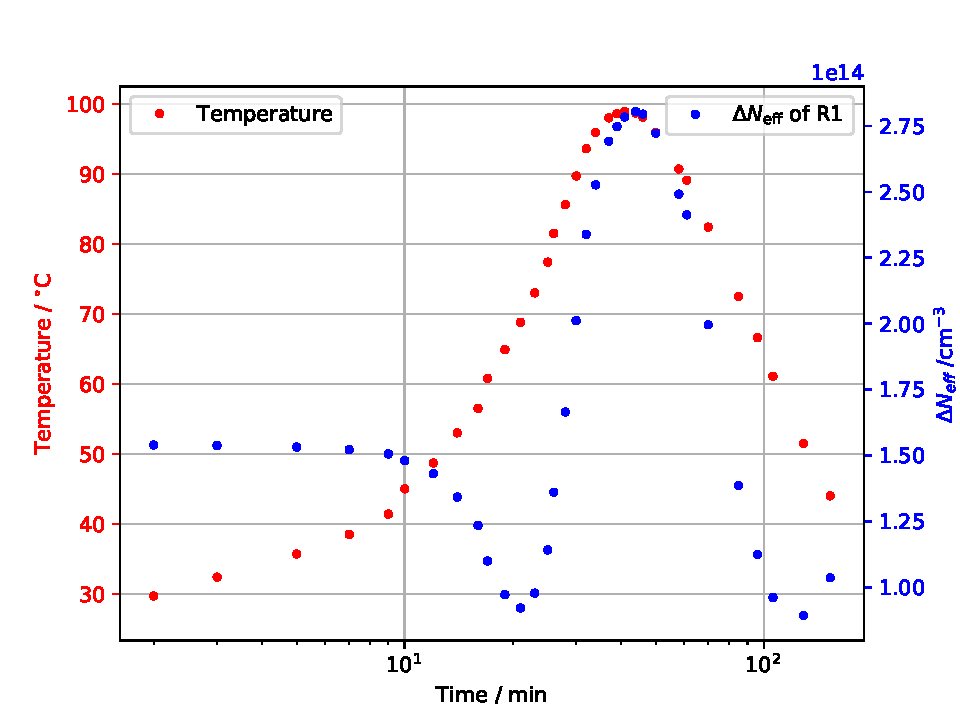
\includegraphics[width=0.49\textwidth]{images/ohnekorrektur.PDF}}
      \subfigure[]{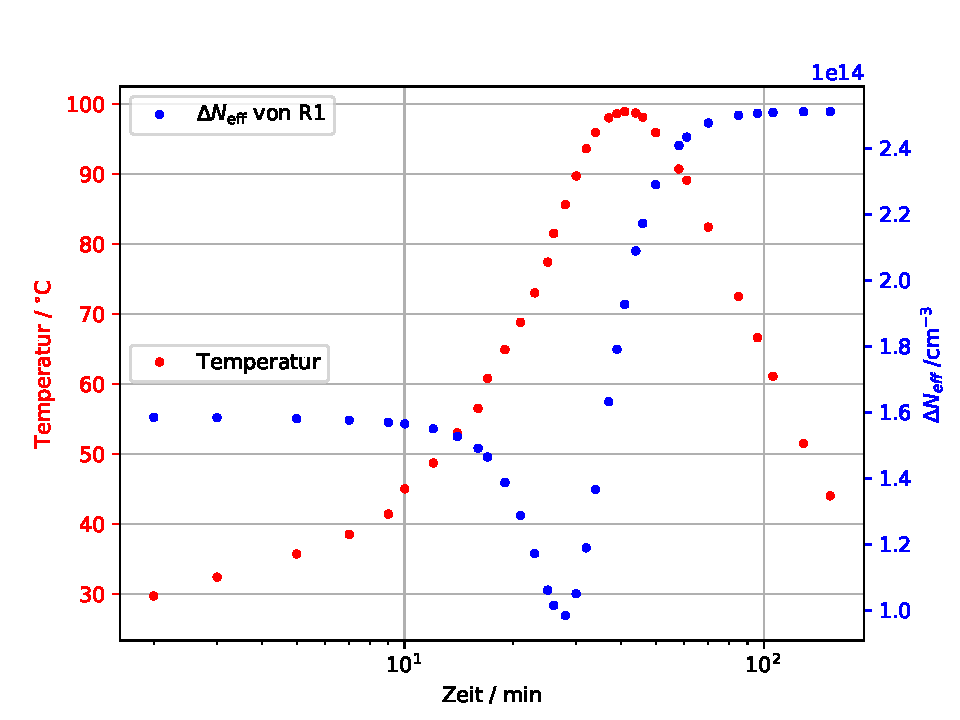
\includegraphics[width=0.49\textwidth]{images/annealingtdata.PDF}}
  \caption{$\Delta N_{eff}$ des Sensors R1 ohne (a) und mit (b) Korrektur nach einer Bestrahlung mit Fluenz $\Phi_{\mathrm{eq}} = \SI{5e15}{\per\centi\meter\squared}.$}
  \end{figure}
\end{frame}

\begin{frame}{Schadensrate mit Korrektur}
  \begin{itemize}
    \item Korrektur funktioniert
    \medskip
    \item Analoger Ansatz für die Schadensrate
    \medskip
    \item Korrektur von $\frac{t}{\tau_{\mathrm{I}}(T)}$ und  $\Theta(T) \cdot t$
    \medskip
    \item Schadensrate kann beim annealing nur sinken
  \end{itemize}
\end{frame}

\begin{frame}{Schadensrate mit Korrektur}
  \begin{figure}
        \subfigure[]{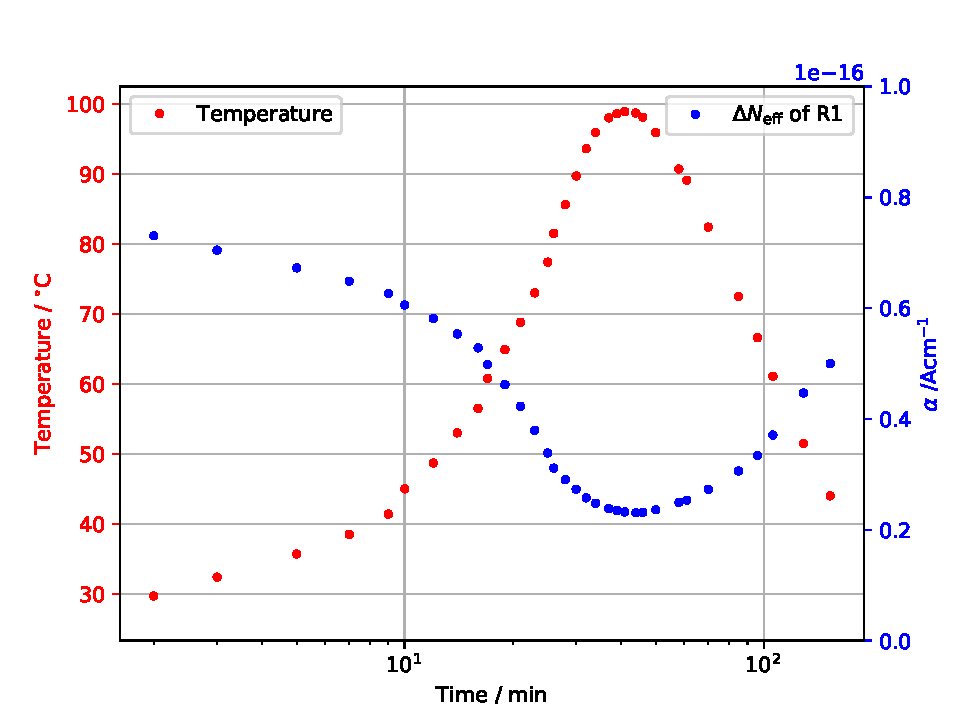
\includegraphics[width=0.49\textwidth]{images/damageohnekorrektur.PDF}}
        \subfigure[]{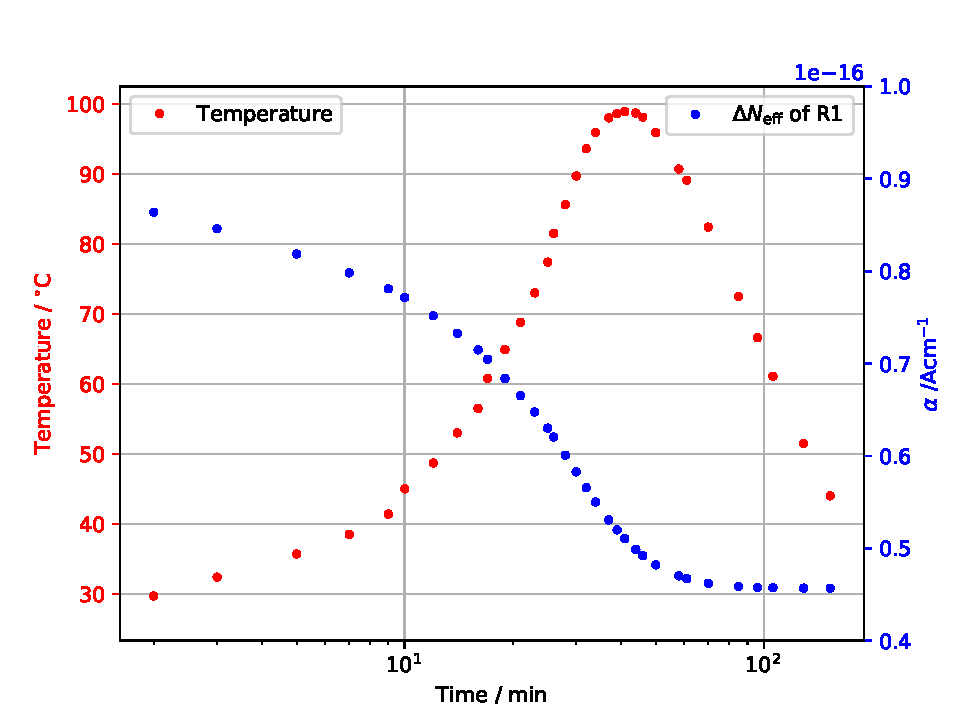
\includegraphics[width=0.49\textwidth]{images/damagekorrektur.PDF}}
  \caption{Schadensrate des Sensors R1 ohne (a) und mit (b) Korrektur}
  \end{figure}
\end{frame}
\end{document}
